\ExamPart{Trắc nghiệm đúng sai}{2}{Thí sinh trả lời từ câu 1 đến câu 2. Trong mỗi ý a), b), c), d) ở mỗi câu học sinh chọn đúng hoặc sai.}

\NQuestion Cho đồ thị hàm số $y=f(x)$ như hình vẽ dưới đây.
\begin{center}
    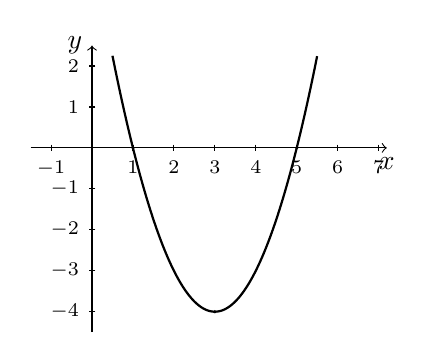
\begin{tikzpicture}[scale=0.52]
    \draw[->] (-1.5,0) -- (7.2,0) node[below] {$x$};
    \draw[->] (0,-4.5) -- (0,2.5) node[left] {$y$};
    \foreach \x in {-1,1,2,3,4,5,6,7}
      \draw (\x,0.08)--(\x,-0.08) node[below] {\scriptsize $\x$};
    \foreach \y in {-4,-3,-2,-1,1,2}
      \draw (0.08,\y)--(-0.08,\y) node[left] {\scriptsize $\y$};
    \draw[smooth, samples=200, domain=0.5:5.5, thick] plot (\x, {(\x-3)*(\x-3)-4});
    \fill (1,0) circle (1.2pt);
    \fill (5,0) circle (1.2pt);
    \fill (3,-4) circle (1.2pt);
\end{tikzpicture}

\end{center}
Xét các khẳng định sau:
\begin{SubQuestions}
  \TFItem{true}{Đồ thị cắt trục hoành tại hai điểm có hoành độ là $1$ và $5$.}
  \TFItem{true}{Trục đối xứng của parabol là đường thẳng $x=3$.}
  \TFItem{false}{Giá trị nhỏ nhất của hàm số bằng $-3$.}
  \TFItem{true}{Bất phương trình $f(x)<0$ có tập nghiệm là $(1;5)$.}
\end{SubQuestions}
\SolutionBlock{Từ đồ thị, parabol mở lên, có hai nghiệm $x=1$, $x=5$, đỉnh là $(3;-4)$ nên giá trị nhỏ nhất là $-4$. Vì vậy a), b), d) đúng; c) sai.}

\NQuestion Trong mặt phẳng tọa độ $Oxy$, cho đường thẳng $d:2x-y+1=0$ và điểm $A(1;2)$. Xét các khẳng định sau:
\begin{SubQuestions}
  \TFItem{true}{Một vectơ pháp tuyến của $d$ là $\vec n=(2;-1)$.}
  \TFItem{false}{Điểm $A$ thuộc đường thẳng $d$.}
  \TFItem{true}{Đường thẳng đi qua $A$ và song song với $d$ có phương trình $2x-y=0$.}
  \TFItem{false}{Khoảng cách từ $A$ đến $d$ bằng $\dfrac{1}{\sqrt5}$.}
\end{SubQuestions}
\SolutionBlock{Đường thẳng $d$ có vectơ pháp tuyến $\vec n=(2;-1)$ nên a) đúng. Thay $A(1;2)$ vào phương trình $d$ được $2\cdot1-2+1=1\ne0$, suy ra $A\notin d$, nên b) sai. Đường thẳng qua $A$ và song song với $d$ có cùng vectơ pháp tuyến, nên có dạng $2x-y+c=0$. Thay $A(1;2)$ vào được $c=0$, vậy phương trình là $2x-y=0$, nên c) đúng. Khoảng cách từ $A$ đến $d$ là
\[
\dfrac{|2\cdot1-2+1|}{\sqrt{5}}=\dfrac{1}{\sqrt5},
\]
nên mệnh đề d) sai.}
